\documentclass{article}
\usepackage[utf8]{inputenc}
\usepackage{graphicx}

\title{MNXB01 Final Project: Group G}
\author{Luo Jia Chen, Emil Verhaard Karlsson, Jing Yi Wang}
\date{October 2022}

\begin{document}
\maketitle

We chose to draw histograms on the temperature dataset of Lund, and we used three different functions to get different results. Two of them, tempOnDay and tempPerDay, were suggested in the project instructions, and the third one tempPerMonth was our own idea. To clean up the data file we used a bash script. Each line of the cleaned data set was then added to a vector in the tempTrender class where it could then be accessed by the member functions mentioned above. This allowed us to easily access the data using substring and stoi in order to use it in our calculations.

\section{Temperature On Day}
\begin{center}
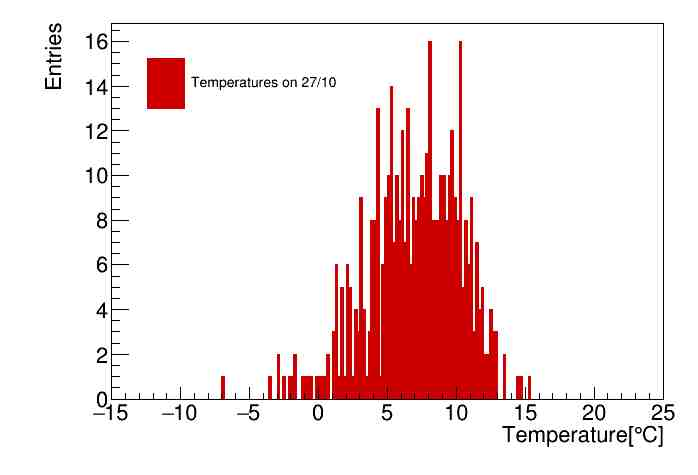
\includegraphics[scale=0.5]{tempOnDay}
\end{center}

The histogram shows the entries of all temperatures measured on the 27th of October from year 1863 to 2020. The histogram was created using the tempOnDay function which iterates through the data and adds an entry to the histogram every time the day and month matched with the requested date.  


\section{Temperature Per Day}
\begin{center}
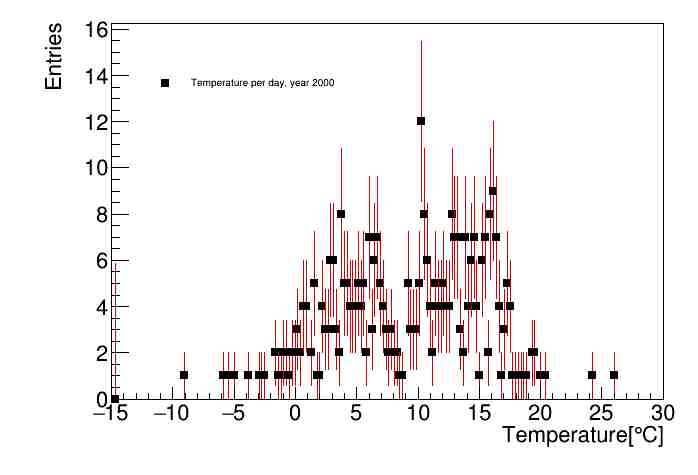
\includegraphics[scale=0.5]{tempPerDay}
\end{center}

The mean temperature of everyday of the year with error bars. 
This is one of the examples given to implement the tempPerDay function.

To do this, we made sure to sort the dates in the dataset in non-decreasing 
order and iterated through to collect the mean temperatures of each day 
in a given year. For example, given the year 2000, we iterated through all 
the dates from the beginning collecting the sum and the number of entries
until the day changed and calculated the mean from there. We then filled the histogram with those values and included the error bar too. 


\section{Temperature Per Month}
\begin{center}
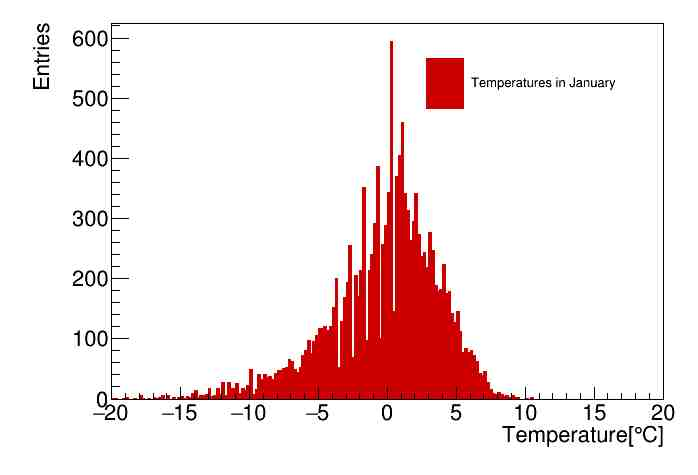
\includegraphics[scale=0.5]{tempPerMonth}
\end{center}

This example was our own idea because it is nice to see the mean temperature 
of a certain month in every year instead of the day as temperatures tend 
to fluctuate more in a month. If we had more time we would have added temperature per season by utilizing the mean temperature per month function written here. It is found that the most popular temperature for the month January is 0 degrees in all years inclusive.

For this, we also iterated through in a similar manner as temp per day but 
we calculated the mean for a month instead and divided by the number of entries. It is notable to mention here that the large white vertical lines are a result of the temperature scale being much smaller than our unit of measurement.

\section{Learnings}
Throughout this process we learned a lot from our mistakes.

Firstly, it was important for us to have an initial meeting to go over how to run
everything and set up the structure of the repository. For instance, reorganize the 
header files, fix the hierarchy, and start the GitHub. It was easier to work together 
and do this on one person's computer because we encountered a lot of issues when 
trying to get started. Specifically, having issues with the paths of import statements, 
compiling the code in general, and running root. Working together to make sure everything worked initially made it easier to spot errors before we added anything on. After this, we divided up histograms and each coded one of them to have a 
different perspective on how to do this. 

In hindsight, we could have added more to our clean up script so that the functions of our 
project could work with all datasets (not just Lund) and even corrupted data that is missing
a column or entry. We should use semicolons for markers not just empty spaces.

We made good use of GitHub in our project by using pull requests and several branches to not only avoid conflicts but branch off each other's work to utilize helper functions. We used this to review each other's work and to maintain a well thought out git history.

\end{document}
